In this section, we compare the selected approaches based on the different perspectives discussed in Section~\ref{sec:method}.
In particular, we analyze and compare each approach based on the dimensions (Section~\ref{sec:dim}), their respective metrics (Section~\ref{sec:met}), types of data (Section~\ref{sec:data}), level of automatization (Section~\ref{sec:auto}) and tool usability (Section~\ref{sec:tools}). 

\subsection{Dimensions}
\label{sec:dim}
%The definition of the \emph{dimensions, and metrics} to assess data quality is a critical activity. 
The linked open data paradigm is the fusion of three different research areas namely \emph{semantic web} to generate semantic connections among data sets,  \emph{world wide web} to make the data available and preferably under an open access license, and \emph{data management} for managing large quantitites of heterogeneous and distributed data.
The selected approaches use quality dimensions taken from any one of these specific areas. 
Previously published literature provides a thorough classification of data quality from a variety of dimensions.
%What kinds of classifications?  
By analyzing the multiple classifications for different quality dimensions provided by \cite{Wand:1996, Wang:1996, Redman:1997, Jarke:2010, Bovee:2003, Naumann:2002}, it is possible to distill a core of set dimensions as: accuracy, completeness, consistency and timeliness. These constitute the focus of the majority of authors Catarci et al. \cite{scannapieco:2002}.
%check citiation.
However, no general agreement on which set of dimensions defines data quality or the exact meaning of each dimension, the same problem occurring in LOD.

As mentioned in Section~\ref{concepts}, data quality assessment involves the measurement of quality dimensions that are relevant to the consumer. %is this really true?? i would guess some of them are relevant to consumers, but many are only relevant for LOD specialists
An initial list of data quality dimensions was first obtained from~\cite{Bizerthesis}.
Thereafter, each approach was analyzed to extract the problem being addressed and later mapped to one or more of the quality dimensions.
For example, the dereferenciability issues, the non-availability of structured data, and content misreportin as mentioned in~\cite{Hogan:2012} were mapped to the dimensions of Completeness as well as Availability.
However, not all the problems present in LOD could be mapped to the initial set of dimensions such as the problem of incoherency or interlinking between datasets or the problem of the alternative representations of the data and its handling i.e. the versatility of the dataset.
As a result , we obtained a further set of quality dimensions, which were particularly relevant for Linked Data.%need more details on how exactly they were derived
Table~\ref{dimensions} shows the complete list of the 25 identified Linked Data quality dimensions along with frequency and occurrence of each dimension. 

There are three visible groups (Table): (a) a set of approaches focusing only on the provenance of the datasets~\cite{Hartig2008, Gamble2011, Shekarpour2010, Golbeck2006, Gil2002, Golbeck2003, Gil2007, Jacobi2011, Bonatti2011, Rula2012}; (b) a set of approaches using more than five dimensions \cite{Bizer, Flemming, Hogan:2012, Mendes} and (c) a set of approaches focusing on very few and specific dimensions  \cite{Bohm, Chen, Gueret, Hogan, Lei, Mostafavi}.
In addition, Provenance, Consistency, Timeliness, Accuracy and Completeness are the most frequently used dimensions. 

\subsection{Metrics}
\label{sec:met}
As defined in Section~\ref{concepts}, data quality metric is a procedure for measuring an information quality dimension.
In general, multiple metrics can be associated with each quality dimension.
In some cases, the metric is unique and the theoretical definition of a dimension coincides with the operational definition of the corresponding metric. 
For this reason, we only make a distinction between theoretical and operational definitions of dimensions when the literature provides multiple metrics.

Table~\ref{metrics} provides a list of the data quality metrics for each of the dimension and classifies it as being either subjective or objective.

%Provenance
In \cite{Hartig2008} the authors determine the measurement of trustworthiness of RDF statements as a value of trust which is either unknown or a value in the [-1,1] interval. 

They do not prescribe and implementation of how to assign a trust value to the statements but instead provide a data provenance model which includes information about the publisher of the dataset, creation method and time of the dataset as well as the publisher along with publication time of possible original sources. 
Therefore the provenance information can be exploited to assess other dimensions such as timeliness or accuracy, which in turn can be merged to provide a unified value of provenance.
In \cite{Gamble2011} the authors suggest the presence of a trusted third party to provide information such as citation count for a publication or global reputation. %what do you mean by global reputation?
Even in this case, the meta information should be provided in advance and the trustworthiness is measured by the reputation dimensions.
In \cite{Shekarpour2010} the author proposes a statistical approach to measure a trust propagation rating between two nodes. 
In \cite{Golbeck2006} the authors infer the trust path from a node A to a node C based on previous trust values given from the path AB and BC. 
However, a pre-established value of trust is needed. 
In \cite{Gil2002} the authors do not address how the trust value is derived. 
Even in this case trustworthiness is calculated possibly as a combination of its popularity, reputation,
and authority. 

\subsection{Type of data}
\label{sec:data}
The ultimate goal of an assessment activity is the analysis of data that, in general, describes real world objects in a format that can be stored, retrieved, and processed by a software procedure, and communicated through a network. 
In LOD, most authors either implicitly or explicitly distinguish three types of data:
\begin{itemize}
\item RDF triple. Given an infinite set $\mathcal{U}$ of URIs (resource identifiers), an infinite set $\mathcal{B}$ of blank nodes, and an infinite set $\mathcal{L}$ of literals, a triple $ \langle s, p, o \rangle \in (\mathcal{U} \cup \mathcal{B})\times \mathcal{U} \times (\mathcal{U} \cup \mathcal{B} \cup \mathcal{L})$ is called an RDF triple; $s$, $p$, $o$ are called, respectively, the subject, the predicate and the object of the triple.
\item Graph. An RDF graph $G$ is a set of RDF triples. A named graph is a pair  $\langle G,u \rangle$, where $G$ is called the default graph and $u\in\mathcal{U}$. [ANDREA we need to underline that a graph is a set of datasource provided by different providers]
\item Dataset. An RDF dataset is a set of default and named graphs = $\lbrace G, (u_1,G_1), (u_2,G_2), ...(u_n,G_n)\rbrace$.
\end{itemize}
%Table~\ref{appfield}

\subsection{Level of automatization}
\label{sec:auto}
%mention that it refers to the involvement of the user, also mention how much knowledge a user requires to use the tool
A set of software tools are needed to support the assessment phase. 
Such tools implement the methodologies and metrics defined in the above described steps. 
Due to the nature of the quality dimensions and related metrics it is possible that some activities are fully or semi automatic or manually realized.
Table~\ref{appfield} shows the level of automatisation for each of the identified tools.

\onecolumn
\begin{landscape}
\begin{longtable}{ | p{3.5cm} | p{0.3cm} | p{0.3cm} | p{0.3cm} | p{0.3cm} | p{0.3cm} | p{0.3cm} | p{0.3cm} | p{0.3cm} | p{0.3cm} | p{0.3cm} | p{0.3cm} | p{0.3cm} | p{0.3cm} | p{0.3cm} | p{0.3cm} | p{0.3cm} | p{0.3cm} | p{0.3cm} | p{0.3cm} | p{0.3cm} | p{0.3cm} | p{0.3cm} | p{0.3cm} | p{0.3cm} | p{0.3cm} | }
\caption{Consideration of data quality dimensions in each of the included approaches.}
\label{dimensions} \\
\hline
Approaches / Dimensions & \begin{sideways}Provenance\end{sideways} & \begin{sideways}Consistency\end{sideways} & \begin{sideways}Timeliness\end{sideways} & \begin{sideways}Accuracy\end{sideways} &  \begin{sideways}Completeness\end{sideways} &  \begin{sideways}Amount of Data\end{sideways} &  \begin{sideways}Availability\end{sideways} &  \begin{sideways}Understandability\end{sideways} & \begin{sideways}Relevancy\end{sideways} &  \begin{sideways}Reputation\end{sideways} &  \begin{sideways}Verifiability\end{sideways} &  \begin{sideways}Interpretability\end{sideways} &  \begin{sideways}Rep. Conciseness\end{sideways} &  \begin{sideways}Rep. Consistency\end{sideways} &  \begin{sideways}Licencing\end{sideways} &  \begin{sideways}Performance\end{sideways} &  \begin{sideways}Objectivity\end{sideways} &  \begin{sideways}Believability\end{sideways} &  \begin{sideways}Response Time\end{sideways} &  \begin{sideways}Security\end{sideways} &  \begin{sideways}Uniformity\end{sideways} &  \begin{sideways}Versatility\end{sideways} &  \begin{sideways}Validity of documents\end{sideways} &  \begin{sideways}Conciseness\end{sideways} &  \begin{sideways}Coherence\end{sideways}\\
\hline 
Bizer et.al.,2009 &  & \tick & \tick & \tick & \tick & \tick & \tick & \tick & \tick & \tick & \tick & \tick & \tick & \tick &  &  & \tick & \tick & \tick & \tick &  &  &  &  & \\ 
\hline
B\"ohm et.al.,2010 &  & \tick &  & \tick &  &  &  &  &  &  &  &  &  &  &  &  &  &  &  &  &  &  &  &  & \\ 
\hline
Chen et.al.,2010  &  & \tick &  &  &  &\tick &  &  &  &  &  &  &  &  &  &  &  &  &  &  &  &  &  &  & \\ 
\hline
Flemming et.al.,2010 &  & \tick & \tick &  &  & \tick & \tick & \tick &  &  & \tick &  &  &  & \tick & \tick &  &  &  &  & \tick & \tick & \tick &  & \\ 
\hline
Gu\'eret et. al,2011 &  &  &  & \tick & \tick &  &  &  &  &  &  &  &  &  &  &  &  &  &  &  &  &  &  &  & \tick\\ 
\hline
Hogan et.al.,2010 &  & \tick &  &  & \tick &  &  &  &  &  &  &  &  &  &  &  &  &  &  &  &  &  &  &  & \\ 
\hline
Hogan et.al.,2012 &  &  &  &  &  &  & \tick &  & \tick &  &  & \tick & \tick & \tick & \tick & \tick &  &  &  &  &  &  &  &  & \\ 
\hline
Lei et.al.,2007 &  & \tick & \tick & \tick &  &  &  &  &  &  &  &  &  &  &  &  &  &  &  &  &  &  &  &  & \\ 
\hline
Mendes et.al., 2012 &  & \tick & \tick &  & \tick &  &  &  &  & \tick &  &  &  &  &  &  &  &  &  &  &  &  &  & \tick & \\ 
\hline
Mostafavi et.al., 2004 &  & \tick &  &  &  &  &  &  &  &  &  &  &  &  &  &  &  &  &  &  &  &  &  &  & \\ 
\hline
F\"urber et.al.,2011 & &  & \tick & \tick & \tick &  &  &  &  &  &  &  &  & \tick  &  &  &  &  &  &  &  &  &  &  & \\ 
\hline
Hartig,2008 & \tick &  &  &  &  &  &  &  &  &  &  &  &  &  &  &  &  &  &  &  &  &  &  &  & \\ 
\hline
Gamble et.al., 2011 & \tick &  &  &  &  &  &  &  &  &  &  &  &  &  &  &  &  &  &  &  &  &  &  &  & \\ 
\hline
Shekarpour et.al., 2008 & \tick &  &  &  &  &  &  &  &  &  &  &  &  &  &  &  &  &  &  &  &  &  &  &  & \\ 
\hline
Golbeck et.al., 2006 & \tick &  &  &  &  &  &  &  &  &  &  &  &  &  &  &  &  &  &  &  &  &  &  &  & \\ 
\hline
Gil et.al., 2002 & \tick &  &  &  &  &  &  &  &  &  &  &  &  &  &  &  &  &  &  &  &  &  &  &  & \\ 
\hline
Golbeck et. al., 2003 & \tick &  &  &  &  &  &  &  &  &  &  &  &  &  &  &  &  &  &  &  &  &  &  &  & \\ 
\hline
Gil et.al., 2007 & \tick &  &  &  &  &  &  &  &  &  &  &  &  &  &  &  &  &  &  &  &  &  &  &  & \\ 
\hline
Jacobi et.al., 2011 & \tick &  &  &  &  &  &  &  &  &  &  &  &  &  &  &  &  &  &  &  &  &  &  &  & \\ 
\hline
Bonatti et. al., 2012 & \tick &  &  &  &  &  &  &  &  &  &  &  &  &  &  &  &  &  &  &  &  &  &  &  & \\ 
\hline
Rula et.al., 2012 & \tick &  &  &  &  &  &  &  &  &  &  &  &  &  &  &  &  &  &  &  &  &  &  &  & \\
\hline
\end{longtable}
\end{landscape}
\twocolumn

\onecolumn
%\begin{table*}[htb]
\begin{longtable}{ | p{3cm} | p{10cm} | >{\centering\arraybackslash}p{2cm}| }
\caption{Comprehensive list of data quality metrics and the type - subjective or objective}
\label{metrics} \\
\hline
\textbf{Dimension} & \textbf{Metric} & \textbf{Type of metric ("S"ubjective/ "O"bjective)} \\
\hline
\multirow{4}{*}{Accuracy} & spurious annotation/representation & O \\
\cline{2-3}
& inaccurate annotation & O \\
\cline{2-3}
& inacurrate labeling and classification & O \\
\cline{2-3}
& detecting poor attributes & O \\
\hline
\multirow{19}{*}{Consistency} & no definitions of entities as being members of disjoint classes & O\\
\cline{2-3}
& valid usage of inverse-functional properties & S \\
\cline{2-3}
& no redefinition of existing properties & S\\
\cline{2-3}
& usage of homogeneous datatypes & O\\
\cline{2-3}
& no stating of inconsistent values for properties & O\\
\cline{2-3}
& duplicate annotation & O\\
\cline{2-3}
& ambiguous annotation & S\\
\cline{2-3}
& duplication representation & O\\
\cline{2-3}
& atypical use of collections, containers and reification & O\\
\cline{2-3}
& use of undefined classes and properties & O\\
\cline{2-3}
& misplaced classes or properties & O\\
\cline{2-3}
& misuse of owl:datatypeProperty or owl:objectProperty & O\\
\cline{2-3}
& use of members of deprecated classes or properties & O\\
\cline{2-3}
& bogus owl:InverseFunctionalProperty values & O\\
\cline{2-3}
& malformed datatype literals & O\\
\cline{2-3}
& literals incompatible with datatype range & O\\
\cline{2-3}
& ontology hijacking & O\\
\cline{2-3}
& misuse of predicates & O\\
\cline{2-3}
& negative dependancies (correlation) among predicates (attribute), negative entity correlation & O\\
\hline
Objectivitiy & no bias or opinion expressed when a data provider interprets or analyses facts & S\\
\hline
\multirow{4}{*}{Timeliness} & stating the most recent and frequency of the validation of the data & S\\
\cline{2-3}
& no inclusion of outdated data & O\\
\cline{2-3}
& dereferencability of all internal and external URIs & O\\
\cline{2-3}
& time inaccurate representation of data &O\\
\hline
\multirow{2}{*}{Believability} & meta-information about the identify of information provider & O\\
\cline{2-3}
& checking source from which information is retrieved & S\\
\hline
\multirow{9}{*}{Completeness} & schema completeness & S\\
\cline{2-3}
& column completeness & O\\
\cline{2-3}
& population completeness & O\\
\cline{2-3}
& data (instance) completeness & S\\
\cline{2-3}
& URI/HTTP: accessibility and dereferencability & O\\
\cline{2-3}
& no structured data available & O\\
\cline{2-3}
& misreported content types & S\\
\cline{2-3}
& number of interlinks & O\\
\hline
\multirow{10}{*}{Understandibility} & human-readable labelling of classes, properties and entities by providing rdfs:label & O\\
\cline{2-3}
& human-readable description of classes, properties and entities by providing an rdfs:comment & O\\
\cline{2-3}
& indication of metadata about a dataset & O\\
\cline{2-3}
& indication of one or more exemplary URIs & O\\
\cline{2-3}
& indication of a regular expression that matches the URIs of a dataset & O\\
\cline{2-3}
& indication of an exemplary SPARQL query & O\\
\cline{2-3}
& indication of some of the vocabularies used & O\\
\cline{2-3}
& operability of HTML documents & S\\
\cline{2-3}
& provision of message boards and mailing lists & O\\
\cline{2-3}
& meta information about the language of web content & O\\
\hline
\multirow{4}{*}{Relevancy} & using meta-information attributes & S\\
\cline{2-3}
& count occurrence of relevant terms within attributes & S\\
%& presence of licensing meta-information like Creative Commons labels & O\\
\cline{2-3}
& sort documents according to their relevancy for a given query & S\\
\cline{2-3}
& existence of links to external data providers: use of external URIs, provide owl:sameAs link & S\\
\hline
\multirow{3}{*}{Verifiability} & stating basic provenance information & S\\
\cline{2-3}
& usage of a dedicated provenance vocabulary & O\\
\cline{2-3}
& usage of digital signatures & O\\
%& traceability and provability & \\
\hline
\multirow{4}{*}{Amount of data} & no. of triples in a dataset & O\\
\cline{2-3}
& no. of internal and external links & O\\
\cline{2-3}
& scope and level of detail - coverage & S\\
\cline{2-3}
& whether the amount of collected data is appropriate & S\\
\hline
\multirow{5}{*}{Interpretability} & use of appropriate language, symbols, units and clear definitions & S\\
\cline{2-3}
& use of self-descriptive formats, identifying objects and terms used to define the objects with globally unique identifiers & O\\
\cline{2-3}
& use of various schema languages to provide definitions for terms & S\\
\cline{2-3}
& avoiding blank nodes & O\\
\cline{2-3}
& dereferenced representations: giving human readable metadata & O\\
\hline
Representational Conciseness & keeping URIs short & O\\
\hline
\multirow{3}{*}{Representational Consistency} & re-use existing terms & O\\
\cline{2-3}
& cherry picking vocabularies & S\\
\cline{2-3}
& provision of data in different representational formats & O\\
\hline
\multirow{11}{*}{Availability} & accessibility of the server & O\\
\cline{2-3}
& accessibility of the SPARQL endpoint & O\\
\cline{2-3}
& accessibility of the RDF dumps & O\\
\cline{2-3}
& usage of dereferencable URIs & O\\
\cline{2-3}
& hosting of stable URIs & O\\
\cline{2-3}
& redirection using the status code 303 See Other & O\\
\cline{2-3}
& dereferencability issues & O\\
\cline{2-3}
& no structured data available & O\\
\cline{2-3}
& misreported content types & S\\
\cline{2-3}
& dereferenced forward links & O\\
\cline{2-3}
& dereference back-links & O\\
\hline
Response time & delay between submission of a request by the user and reception of the response from the system & O\\
\hline
Security & & \\
\hline
\multirow{4}{*}{Uniformity} & usage of an established format & O\\
\cline{2-3}
& stating the content-types as specifically as possible & O\\
\cline{2-3}
& usage of established vocabularies & O\\
\cline{2-3}
& referencing of established URIs  & O\\
\hline
\multirow{6}{*}{Versatility} & provision of the data in various formats & O\\
\cline{2-3}
& provision of the data in various languages & O\\
\cline{2-3}
& application of content negotiation & O\\
\cline{2-3}
& correct interpretation of the accept-headers sent & O\\
\cline{2-3}
& human-readable indication of a SPARQL-endpoint & O\\
\cline{2-3}
& machine-readable indication of a SPARQL-endpoint & O\\
\hline
\multirow{4}{*}{Validity of documents} & no syntax errors & \\
\cline{2-3}
& exclusive usage of defined classes and properties & O\\
\cline{2-3}
& no usage of deprecated classes and properties & O\\
\cline{2-3}
& usage of proper datatypes & O\\
\hline
\multirow{7}{*}{Licensing} & machine-readable indication of a licence & O\\
\cline{2-3}
& human-readable indication of a licence & O\\
\cline{2-3}
& permitted reproduction of data & O\\
\cline{2-3}
& permitted distribution of data & O\\
\cline{2-3}
& permitted modification and redistribution of data & O\\
\cline{2-3}
& no attribution needed & O\\
\cline{2-3}
& no Copyleft / Share Alike needed & O\\
\hline
\multirow{7}{*}{Performance} & machine-readable indication of one or more RDF dumps & O\\
\cline{2-3}
& human-readable indication of one or more RDF dumps & O\\
\cline{2-3}
& usage of Slash-URIs when providing a large amount of data & O\\
\cline{2-3}
& low latency & O\\
\cline{2-3}
& high throughput & O\\
\cline{2-3}
& maintenance of the performance no matter the load & O\\
\cline{2-3}
& avoiding use of prolix RDF features & O\\
\hline
\multirow{2}{*}{Conciseness} & schema level : intensional conciseness - does not contain redundant attributes & O\\
\cline{2-3}
& data level : extensional conciseness - does not contain redundant objects & O\\
\hline
\multirow{6}{*}{Provenance} & using provenance information and trust annotations in SW based social networks & S\\
\cline{2-3}
& a trust value based on the meta-information about the provenance of the data which can be either unknown or a value in the interval [-1,1]  & S\\
\cline{2-3}
& construction of decision networks informed by provenance graphs & O\\
\cline{2-3}
& statistical techniques and an aggregation algorithm based a weighting mechanism that utilizes fuzzy logic for modeling & O\\
\cline{2-3}
& use of annotations by many individuals & O\\
\hline
%\end{tabular}
%\end{table*}
\end{longtable}
\twocolumn

\onecolumn
\begin{landscape}
\begin{savenotes}
\begin{table*}
\caption{Qualitative evaluation of frameworks} \label{appfield}
\begin{tabular}{ p{2.3cm} c p{5cm}  c  p{0.9cm} l p{1cm} l p{0.7cm} l  p{4.27cm} }
\hline
\textbf{Paper} & {\textbf{Application}} & \textbf{Goal} & \multicolumn{4}{c}{\textbf{Type of data}} & \multicolumn{3}{c}{\textbf{Degree of automation}} & \textbf{Tool support} \\
%\cline{2-4}
\hline
 & \textbf{G}eneral/\textbf{S}pecific &  & \textbf{Triple} & \textbf{Resource} & \textbf{Several resources} & \textbf{Entire LOD Cloud} & \textbf{Manual} & \textbf{Semi-automated} & \textbf{Automated} & \\
\hline
Gil et.al., 2002 & G & Approach to derive an assessment of a data source
based on the annotations of many individuals & \tick & \tick & - & - & - & \tick & - & \tick~\url{http://trellis.isi.edu/}\\
\hline
Golbeck et.al., 2003 & G & Trust networks on the semantic web & - & \tick & - & - & - & - & - & - \\
\hline
Mostafavi et.al., 2004 & S & Spatial data integration & \tick & \tick & - & - & - & - & - & - \\
\hline
Golbeck, 2006 & G & Algorithm for computing personalized trust recommendations using the provenance of existing trust annotations in social networks & - & - & \tick & \tick & - & - & - & - \\
\hline
Gil et.al., 2007 & S & Trust assessment of web resources & - & \tick & - & - & - & - & - & - \\
\hline
Lei et.al., 2007 & S & Assessment of semantic metadata & \tick & \tick & - & - & - & - & - & - \\
\hline
Hartig, 2008 & G & Trustworthiness of Data on the Web & \tick & - & - & - & - & \tick & - & \tick~\url{http://trdf.sourceforge.net/} \\
\hline
Bizer et.al., 2009 & G  & Information filtering & \tick & \tick & \tick & -  & \tick &  - & - & \tick~\url{http://www4.wiwiss.fu-berlin.de/bizer/wiqa/} \\
\hline
B\"ohm et.al., 2010 & G  & Data integration & \tick & \tick & - & - &  & \tick & -  & \tick~\url{https://www.hpi.uni-potsdam.de/naumann/sites/lodprof/ProLOD/ProLOD.html} \\
\hline
Chen et.al., 2010  & G  & Generating semantically valid hypothesis & \tick & \tick & - & - & - & - & - & - \\
\hline
Flemming et.al., 2010 & G  & Assessment of published data & \tick & \tick & - & - & - & \tick & - & \tick~\url{http://linkeddata.informatik.hu-berlin.de/LDSrcAss/} \\
\hline
Hogan et.al., 2010 & G &Assessment of published data by identifying RDF publishing errors and providing approaches for improvement & \tick & \tick & \tick &\tick & - & \tick & - & \tick~\url{http://www.w3.org/RDF/Validator/} \\
\hline
Shekarpour et.al., 2010 & G & Method for evaluating trust & - & - & \tick & \tick & - & - & - & - \\
\hline
F\"urber et.al., 2011 & G & Assessment of published data & \tick & \tick & - & - & - & - & - & - \\
\hline
Gamble et.al., 2011 & G & Application of decision networks to quality, trust
and utility assessment & - & - & \tick & \tick & - & - & - & - \\
\hline
Jacobi et.al., 2011 &  G & Trust assessment of web resources & - & \tick & - & - & - & - & - & - \\
\hline
Bonatti et.al., 2011 &  G & Provenance assessment for reasoning & \tick & \tick & - & - & - & - & - & - \\
\hline
Gu\'eret et.al., 2012 & S & Assessment of quality of links & - & - & - & \tick & - & - & \tick & \tick~\url{http://qa.linkeddata.org/frontend/} \\
\hline
Hogan et.al., 2012 & G & Assessment of published data & \tick & \tick & \tick &\tick & - & - & - & - \\
\hline
Mendes et.al., 2012 & S & Data integration & \tick & - & - & - & \tick & - & - & \tick~\url{http://www4.wiwiss.fu-berlin.de/bizer/sieve} \\
\hline
Rula et.al., 2012 & G & Assessment of time related quality dimensions & \tick & \tick & \tick & - & - & - & - & - \\
\hline
\end{tabular}
\end{table*}
\end{savenotes}
\end{landscape}
\twocolumn

\subsection{Comparison of tools}
\label{sec:tools}
In this section, we analyze three particular tools, namely, Flemmings Data Quality Assessment Tool, Sieve and LODGRefine to assess their usability for data quality assessment. 
In particular, we compare them in terms of their ease of use, level of user interaction, applicability in terms of data quality assessment and discuss their pros and cons.
%describe, user involvement, screenshot
\paragraph{Flemmings Data Quality Assessment Tool.}
The data quality assessment tool proposed in~\cite{Flemming}, is a simple user interface\footnote{available only in German at \url{http://linkeddata.informatik.hu-berlin.de/LDSrcAss/datenquelle.php}}, where a user first needs to specify the name, URI and three entities of a particular data source. 
Then, via a series of steps, the user is ultimately provided with a score out of 100 indicating the quality of the dataset. 

After specifying the dataset details, the user is given an option of assigning weights to each of the pre-defined data quality metrics. 
There are two choices for assigning the weights: (a) assigning a weight of 1 to all the metrics or (b) choosing the pre-defined exemplary weight of the metrics defined for a data source.
% from the view of a semantic search engine consisting of a crawler, validator, derived statements and indexers. 
In the next step, the user is asked to answer a series of questions regarding the datasets, which are important indicators of the data quality of Linked Open Datasets and those which cannot be quantified. 
For example, questions such as the use of stable URIs, the number of obsolete classes and properties and whether the datasets provides a mailing list. 
Next, the user is presented with a list of dimensions and metrics and is allowed to specify yet again a set of weightings for each of them.
This step is important especially for those indicators for which no formalization of the quantification exists (indicated against each of the metric). 
Also, those metrics which are assigned a weight of 0 are are not included in the final assessment.
Each metric is provided with 2 input fields: first showing the assigned weights and second showing the calculated value. 

At the end, the user is presented with a score, out of 100, based on the answers of all the questions, which is the data quality score.
Additionally, the rating of each dimension and the total weight (out of 11 on account of 11 dimensions used in the assessment) is presented based on the user input from the previous step. 
Figure~\ref{fig:flemmingtool} shows an excerpt of the tool showing the result of assessing the quality of DBpedia with a score of 64 out of 100. 

\begin{figure}[htb]
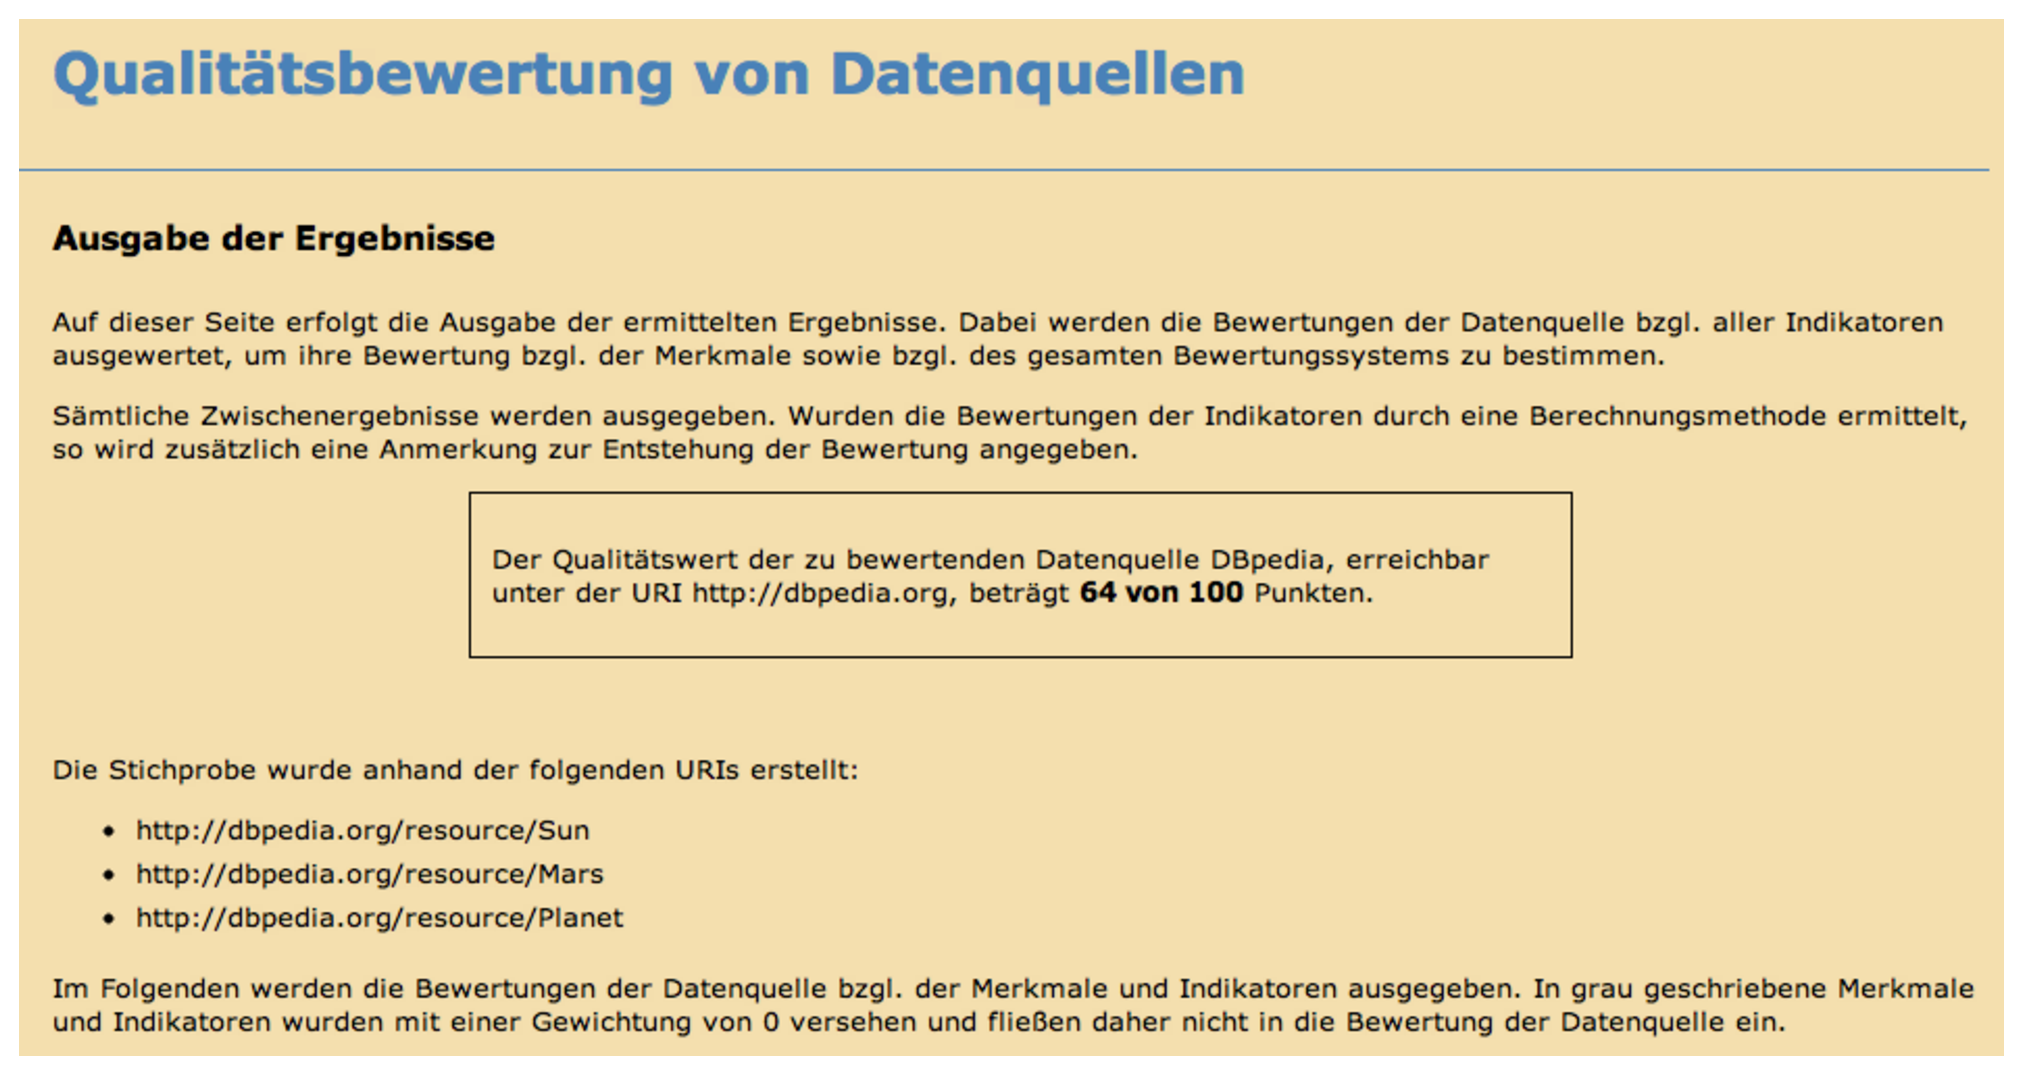
\includegraphics[width=3.5in]{Flemmingtool.pdf}
\caption{Excerpt of the Flemmings Data Quality Assessment tool showing the result of assessing the quality of DBpedia with a score of 64 out of 100.}
\label{fig:flemmingtool}
\end{figure}

On the one hand, the tool is easy to use with the form-based questions and adequate explanation for each step. 
Also, the assigning of the weights for each metric and the calculation of the score is straightforward and easy to adjust for each of the metrics. 
However, on the other hand, this tool has a few drawbacks: (1) the user needs to have adequate knowledge about the dataset in order to correctly assign weights for each of the metrics; (2) it does not drill down to the root cause of the proposed data quality problem and (3) some of the main quality dimensions are missing from the analysis such as accuracy, completeness, provenance, consistency, conciseness and relevancy as some could not be quantified and were not perceived to be true quality indicators. 

\paragraph{Sieve.}

\paragraph{LODGRefine.}
LODGRefine\footnote{\url{http://code.zemanta.com/sparkica/}} is a LOD-enabled version of Google Refine, which is an open source tool for working with messy data. 
Although this tool is not focused towards data quality assessment per-say, it is very powerful in performing preliminary cleaning or refining of raw data. 

Using this tool, one is able to import several different file types of data (CSV, Excel, XML, RDF/XML, N-Triples or even JSON) and then perform cleaning over it. 
In particular, it helps in detecting duplicates, discovering patterns (e.g. alternative forms of abbreviations), spotting inconsistencies (e.g. trailing white spaces), finding blank cells and similar errors. 

Additionally, this tool allows users to reconcile data, that is to connect a dataset to existing vocabularies such that it gives meaning to the field values. 
This feature thus assists in assessing as well as improving the data quality, in particular the interpretability, of a dataset. 
Reconciliations to Freebase\footnote{\url{http://www.freebase.com/}} helps mapping ambiguous textual values to precisely identified Freebase entities. 
Reconciling using Sindice or based on standard SPARQL or SPARQL with full-text search is also possible\footnote{\url{http://refine.deri.ie/reconciliationDocs}}.
Moreover, it is also possible to extend the reconciled data with DBpedia as well as exporting the data as RDF using this tool, which adds to the uniformity of the dataset.

LODGRefine is easy to download and install as well as to upload and perform basic cleansing steps on raw data.
The features of reconciliation, extending the data with DBpedia, exporting the data as RDF add to the usability, interpretability and uniformity of the dataset.
However, this tool has a few drawbacks: (1) the user is not able to perform detailed high level data quality analysis utilizing the various quality dimensions using this tool; (2) performing cleansing over a large dataset is time consuming as the tool follows a column data model and thus the user must perform transformations per column.
%Figure
%Drawback
 
\subsection{Summary and comparison of selected approaches}
%No, of papers from each year or each conference/journal - quantitative analysis

\section{Proposed Linked Data quality assessment steps}
% Which papers follow which steps
% Introduce the tools mentioned in Step 4
%Lay-users, tech users and domain experts
%
%A data quality assessment methodology is defined as the process of evaluation if a piece of data meets in the information consumers need in a specific use case~\cite{Bizer}.
%The process involves measuring the quality dimensions that are relevant to the user and comparing the assessment results with the users quality requirements.
%
%The steps of the assessment phase are:
%\begin{itemize}
%\item data analysis, which examines data schemas and performs interviews to reach a
%complete understanding of data and related architectural and management rules;
%\item DQ requirements analysis, which surveys the opinion of data users and administrators
%to identify quality issues and set new quality targets;
%\item identification of critical areas, which selects the most relevant databases and data
%flows to be assessed quantitatively;
%\item process modeling, which provides a model of the processes producing or updating
%data;
%\item measurement of quality, which selects the quality dimensions affected by the quality
%issues identified in the DQ requirements analysis step and defines corresponding
%metrics; measurement can be objective when it is based on quantitative metrics, or
%subjective, when it is based on qualitative evaluations by data administrators and
%users.
%\end{itemize}
%Note that in all the steps of the assessment phase, a relevant role is played by metadata
%that store complementary information on data for a variety of purposes, including
%data quality. Metadata often provide the information necessary to understand data
%and/or evaluate them.

As defined in Section~\ref{concepts}, a data quality assessment methodology is defined as the process of evaluation if a piece of data meets in the information consumers need in a specific use case~\cite{Bizer}.
In each of the identified approaches, we extracted the methodology that they followed to assess the quality of a dataset. 
Based on our analysis of the existing approaches as well as the evaluated tools, we identified a series of steps followed by majority of the approaches. 
We then adapted and revised the steps to align them with the data quality assessment process performed particularly for LOD as follows: 
\begin{enumerate}
\item Requirements analysis (optional)
\item Data Quality Checklist
\item Statistics and low-level analysis
\item Aggregated and higher level metrics
\item Comparison (optional)
\item Interpretation
\end{enumerate}

Table~\ref{metricsteps} comprises of the steps involved in the data quality assessment process. 
We also provide the input and output for each step along with a list of tools that would support at each step. 
Moreover, we identify the user involvement for each of the steps, that is, we identify whether the tool is automated, semi-automated or manual.
%The "Assessment steps" measures the quality of data collections along relevant quality dimensions; in particular the measurement of quality dimensions is provided by a set of metrics defined for each dimension. 

We now describe each of the steps in detail. 
\paragraph{\textbf{Requirements analysis (optional).}}
The multidimensionality of the information quality makes it dependent on a number of factors that can be achieved by the analyses of the user requirements. 
Thus, the use case in question is highly important when assessing the quality of a dataset.
This step is optional since it is not always provided in LOD related approaches and not all users necessarily have a use case in mind when assessing the quality of the dataset.
In other words, a user might just want to find out the completeness of a dataset and will not have any particular use case for that particular dataset.

\emph{Input.} As the input is the use case specified by the user with the aim of assessing the data quality of a particular dataset.

In this step, we identify two types of users: (a) those who know the problem with their dataset and (b) those who don't. 
Both users, however, are interested in finding the \emph{fitness of use} for their dataset.

\paragraph{\textbf{Data Quality Checklist.}}
After specifying a use case or after deciding to assess the quality of a dataset, the user then is presented with a list of data quality dimensions but only those that do not have a specified statistical metric available. 
That is those dimensions which can perhaps be measured qualitatively. 

\emph{Input.} In this step, a checklist of data quality dimensions are presented to the user, but only those dimensions which call upon a boolean answer. 
That is, the user has to either tick which dimensions are present or provide a 0 (no) if it not present or 1(yes) if it is present.

\emph{Output.} The output of this step is the result of the evaluation of these boolean dimensions, that is, a sum of 0's(no) or 1's(yes) which add to the final data quality assessment report. 

\emph{Tool Support.} Flemmings Data Quality Assessment tool\footnote{\url{http://linkeddata.informatik.hu-berlin.de/LDSrcAss/}} includes such questions in the process of data quality assessment.
For example, questions such as whether the datasets provides a message board or a mailing list pointing to the Comprehensibility dimension are asked to the user. 
Thus, the user involvement is entirely manual where the user must have knowledge about the details of the dataset to answer these questions.

\paragraph{\textbf{Statistics and low-level analysis.}}
This step performs basic statistical and low-level analysis on the dataset.
Generic statistics on the dataset are calculated. 

\emph{Input.} The input for this step is the dataset itself. 

\emph{Output.} The output is a statistical overview of the dataset. 
That is, it provides generic statistics on the dataset based on certain pre-defined heuristics.

\emph{Tool Support.} LODStats\footnote{\url{http://stats.lod2.eu/}} and LODGRefine\footnote{\url{http://code.zemanta.com/sparkica/}} are two tools identified to provide such basic analysis on a dataset.
LODStats gathers comprehensive statistics about a dataset available as RDF. 
It helps to know the structure, coverage and coherence of the data. 
It provides 32 different statistics such as property usage, vocabulary usage, datatypes used, average length of string literals, number of interlinks, to name a few. 
Thus, it helps to provide important insights with regard to the expected quality.
%screenshot?

LODGRefine, on the other hand, helps users import their dataset and presents them an overview of the possible short-comings of the dataset. 
For example, characteristics such as Completeness,  Interpretability of the column headers or Consistency is evident to the user. 
Moreover, it allows easy data cleansing mechanisms by performing transformations on a large amount of data at once. 
Additionally, LODGRefine also provides the functionality of reconciling data with Freebase\footnote{\url{http://www.freebase.com/}} or DBpedia, thus increasing the Coherency of the dataset.
Both these tools work automatically once a user uploads their dataset.

\paragraph{\textbf{Aggregated and higher level metrics.}} 
In this step, 

\emph{Input.} This step includes all the dimensions that are not included in the Data Quality Checklist step, that is those dimensions which can be measured quantitatively.   

\emph{Output.} 
As an output, a single metric or a combination of them produces a value within the range [0;1]. 

\emph{Tool Support.} 
There are a number of tools we identified that perform the tasks involved in this step. 
WIQA~\cite{Bizer} is a information quality assessment framework which allows users to apply a wide range of policies to filter information. 
When a user browses the web, WIQA runs in the background and analyses the web pages. 
It then extracts structured information from the page such as the quality-related as well as basic provenance information and stores it in a local repository. 
This stored information can then be filtered using quality-based information filtering policies to show only information matching the policy. 
These policies take into account the different types of quality-related meta-information available in the dataset. 
It is a semi-automated tool that can help to perform 

ProLOD~\cite{Bohm} is another tool that works semi-automatically  in which the triples of a dataset is stored in a relational database. 
The triples are then enriched with data type and pattern information and are divided into clusters.
Then the user can select a particular cluster, the facts and statistics of which is presented in detail. 
The tool helps in discovering poor attributes (i.e. those that do not contain useful values for most data entries), occurrence dependencies (e.g. book entity from a media cluster), negative dependencies (e.g. negative associations between the predicates author and developer in a media closer) as well as misusage among predicates.

Flemmings Data Quality Assessment Tool~\cite{Flemming} also supports in calculating higher level metrics 
%Ex: WIQA, ProLOD, Flemming, LinkQA, W3C's RDF Validator + other validators, Sieve, EvoPat, ORE


\paragraph{\textbf{Comparison (optional).}}
Used when the resulted measurements provided in step "Aggregated and higher level metrics" are compared to reference values such as previous values from dataset in the same domain or gold standard values, in order to enable a diagnosis of quality. 

\emph{Input.} 
"Target/derived dataset (eg. Geonames)
Assessment results from step 2 and 4
Original dataset (eg. OpenStreetMap)"

\emph{Output.} 
evaluation of the representation
evaluation between datasets in the same domain"

\emph{Tool Support.} 
%Not come across any tools, highly domain dependant

\paragraph{\textbf{Interpretation.}}
Gives an interpretation to the results obtained from step Data Quality Checklist.

\emph{Input.} 
Assessment results from Step 2 and 4

\emph{Output.} 
Explanation of the results

\emph{Tool Support.} 
%Ex in WIQA

\begin{table*}[htb]
\caption{Data quality assessment steps}
\label{metricsteps}
\begin{tabular}{ | p{2cm} | p{3.3cm} | p{3.7cm} | p{1.5cm} | c | c | c | }
\hline
\textbf{Steps} & \textbf{Input} & \textbf{Output} & \textbf{Tool support} & \multicolumn{2}{c}{\textbf{User involvement }} & \cr
\hline
& & & & \textbf{Automated} & \textbf{Semi-automated} & \textbf{Manual} \\
\hline
\textbf{Requirements analysis (optional)} & Assessment of data quality, 2 types of users: \begin{itemize} \item who know the problem with their dataset \item who do not know the problem with their dataset \end{itemize} & - & - & - & - & - \\
\hline
\textbf{Data quality checklist} & Checklist of dimensions which have a binary evaluation & Results of the evaluation - 0 (no) or 1 (yes) & Flemming et al., 2010  & - & - & - \\
\hline
\textbf{Statistics and low level analysis} & Dataset & \multirow{3}{*}{Overview statistics of the dataset} & LODStats & \tick & - & - \\
\cline{4-7}
 & & & LODGRefine & \tick & - & - \\
\hline
\textbf{Aggregated and higher level metrics} & Dimensions not included in Step 2 & \multirow{8}{3cm}{Results of the evaluation of these dimensions in a range from 0 to 1}
 & WIQA & - & \tick & -  \\
 \cline{4-7}
 & & & ProLOD & - & \tick & - \\
 \cline{4-7}
 & & & Flemming et al., 2010 & - & \tick & - \\
 \cline{4-7}
 & & & LinkQA & \tick & - & - \\
 \cline{4-7}
 & & & W3C's RDF Validator & - & \tick & - \\
 \cline{4-7}
 & & & Sieve & - & - & \tick \\
 \cline{4-7}
 & & & EvoPat & - & - & \tick \\
 \cline{4-7}
 & & & ORE & - & \tick & - \\
\hline
\textbf{Comparison (optional)} & \begin{itemize} \item Target/derived dataset \item Assessment results from step 2 and 4 \item Original dataset \end{itemize} & \begin{itemize} \item Evaluation of the representation \item Evaluation between datasets in the same domain \end{itemize} & - & - & - & - \\
\hline
\textbf{Interpretation} & Assessment results from Step 2 and 4 & Explanation of the results & WIQA & - & - & \tick \\
\hline
\end{tabular}
\end{table*}
